\section{Análisis del comportamiento del modelo}
En esta sección se estudia el comportamiento del modelo de El Niño y su sensibilidad a los parámetros que lo definen. El análisis se basa en una solución numérica obtenida mediante el método de Euler explícito en la sección anterior, tomando un paso temporal $h=0.00005$ que garantiza una solución estable y precisa. Además, se realiza una simulación del sistema durante 60 meses y se proponen como indicadores la severidad estacional de las precipitaciones y el desfase temperatura-precipitación. Los indicadores de esta sección se calculan utilizando el último ciclo anual, correspondiente al intervalo $48 \le t \le 60$ meses.

\begin{itemize}
    \item Se define la severidad estacional de las precipitaciones como:
    \begin{equation}
    S_P = \frac{P_{\max} - P_{\min}}{P_{\mathrm{med}}},
    \end{equation}
    donde $P_{\max}$, $P_{\min}$ y $P_{\mathrm{med}}$ (promedio) se calculan utilizando únicamente el último ciclo anual.

    \item El desfase temperatura-precipitación se define como el tiempo transcurrido desde el máximo de $T$ hasta el máximo posterior de $P$:
    \begin{equation}
    \Delta t_{TP} = t_{P,\max} - t_{T,\max}
    \end{equation}
\end{itemize}

\subsection{Indicadores resultantes con parámetros nominales}
Para comenzar, graficamos las tres funciones $T(t)$, $H(t)$, $P(t)$ usando los valores nominales dados por la tabla de la sección 1.1 para todo el período de 60 meses.


\begin{figure}[H]
    \centering
    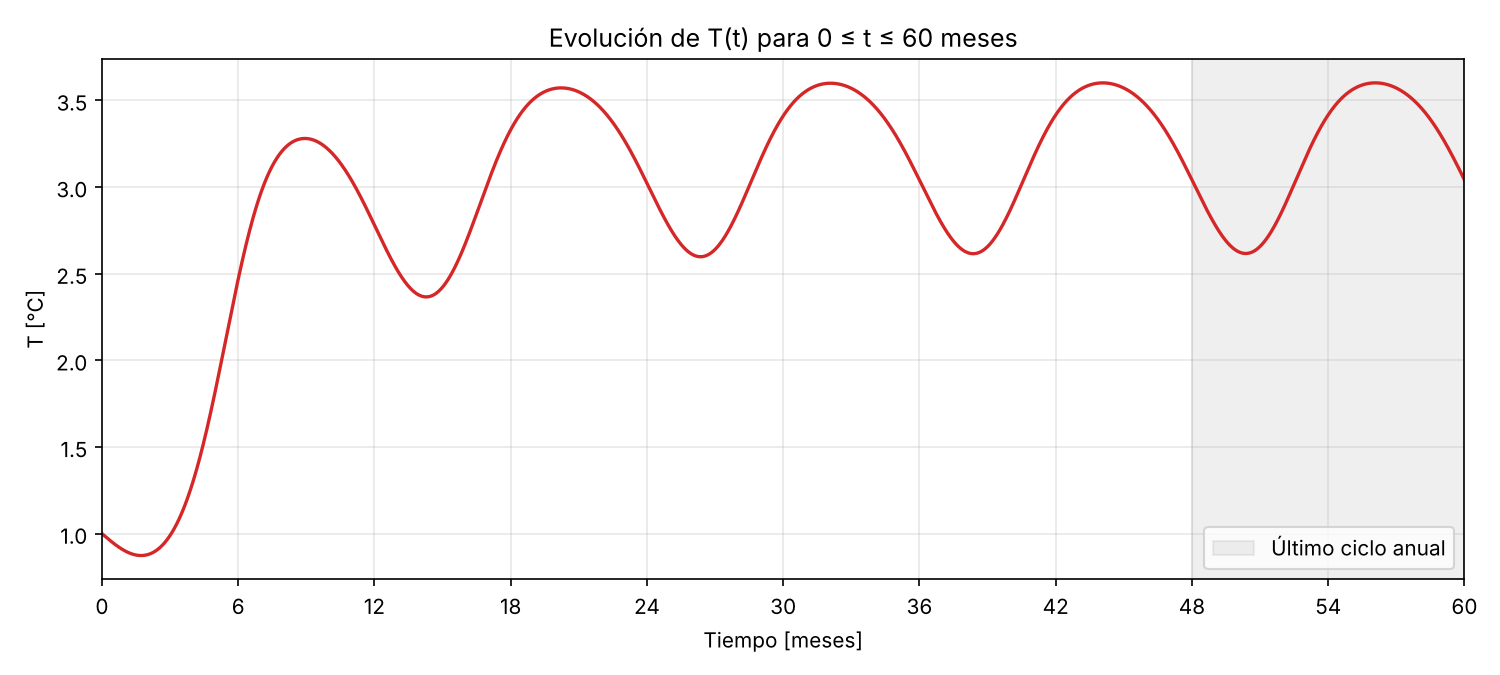
\includegraphics[width=0.75\linewidth]{graficoT60.png}
    \caption{Evolución de $T(t)$ para $0 \le t \le 60$ meses.}
    \label{fig:T60}
\end{figure}

\begin{figure}[H]
    \centering
    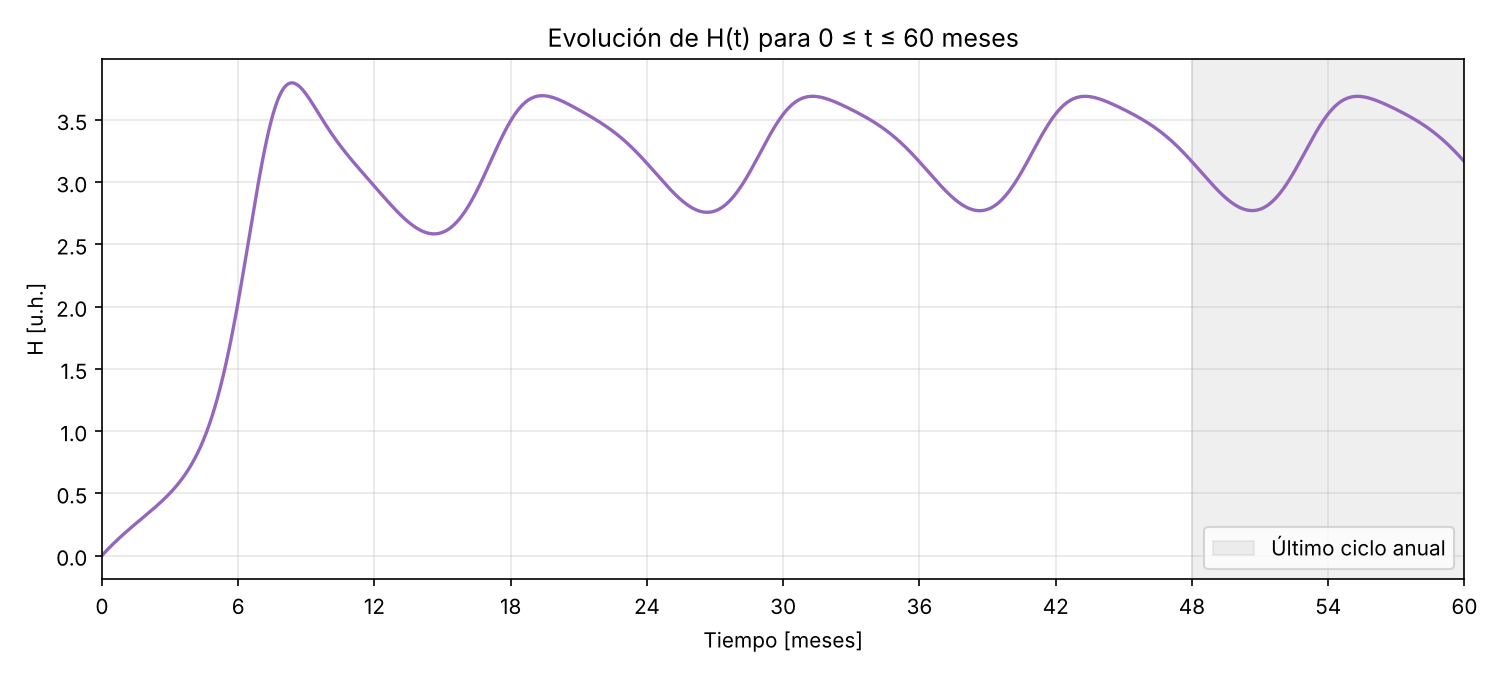
\includegraphics[width=0.75\linewidth]{graficoH60.png}
    \caption{Evolución de $H(t)$ para $0 \le t \le 60$ meses.}
    \label{fig:H60}
\end{figure}

\begin{figure}[H]
    \centering
    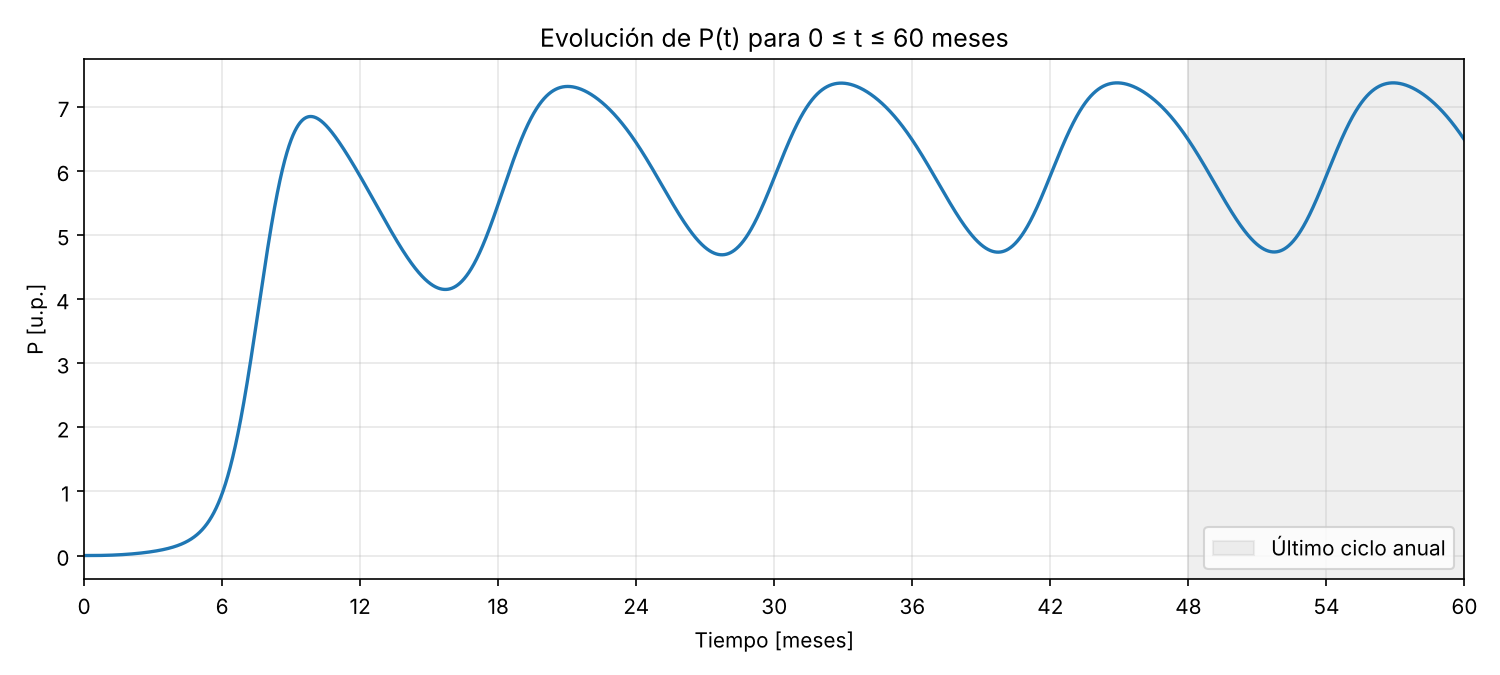
\includegraphics[width=0.75\linewidth]{graficoP60.png}
    \caption{Evolución de $P(t)$ para $0 \le t \le 60$ meses.}
    \label{fig:P60}
\end{figure}

Para el cálculo de los indicadores, se tendrán en cuenta los valores obtenidos en el último ciclo anual de $48 \le t \le 60$ meses.

\begin{figure}[H]
    \centering
    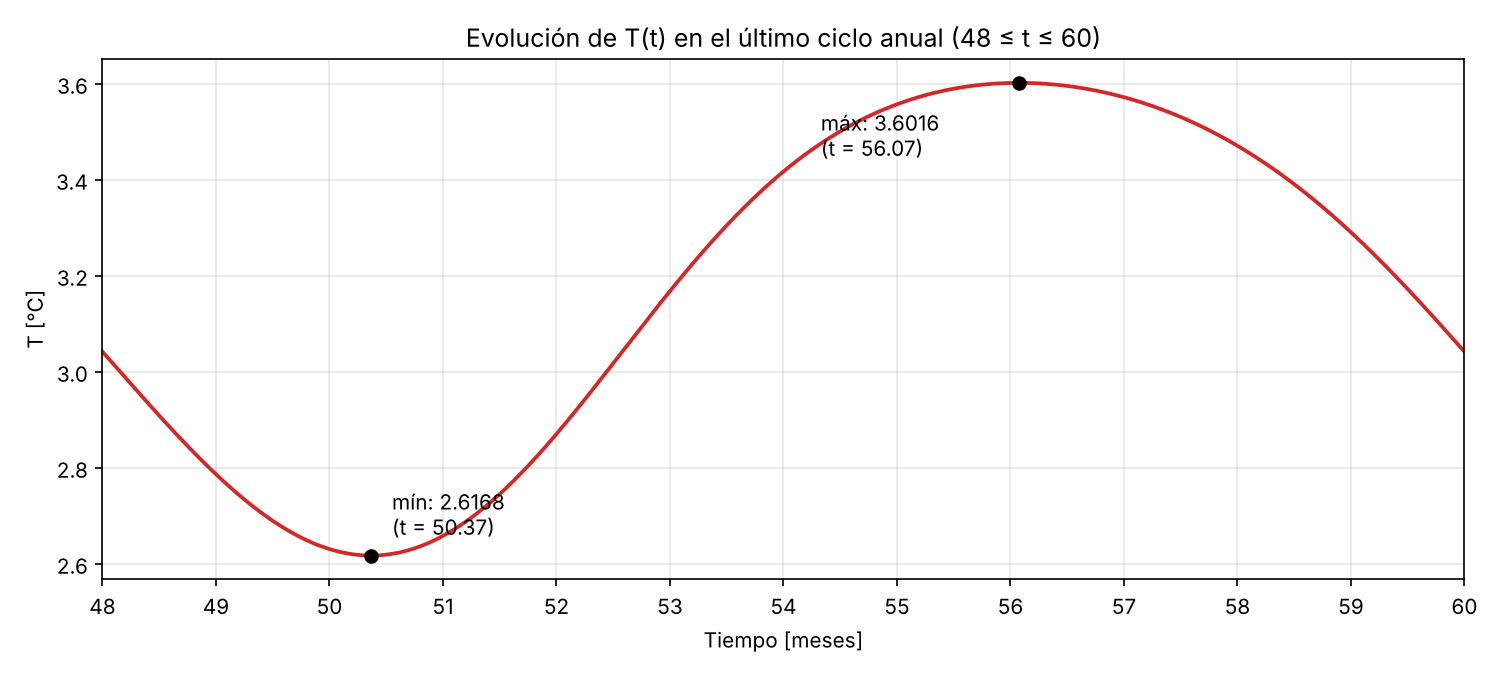
\includegraphics[width=0.75\linewidth]{graficoT.png}
    \caption{Evolución de $T(t)$ para $48 \le t \le 60$ meses.}
    \label{fig:T}
\end{figure}

A partir de la Figura 4, el máximo de la temperatura se alcanza en
$t_{T,\max} = 56.07\ \text{meses}$.


\begin{figure}[H]
    \centering
    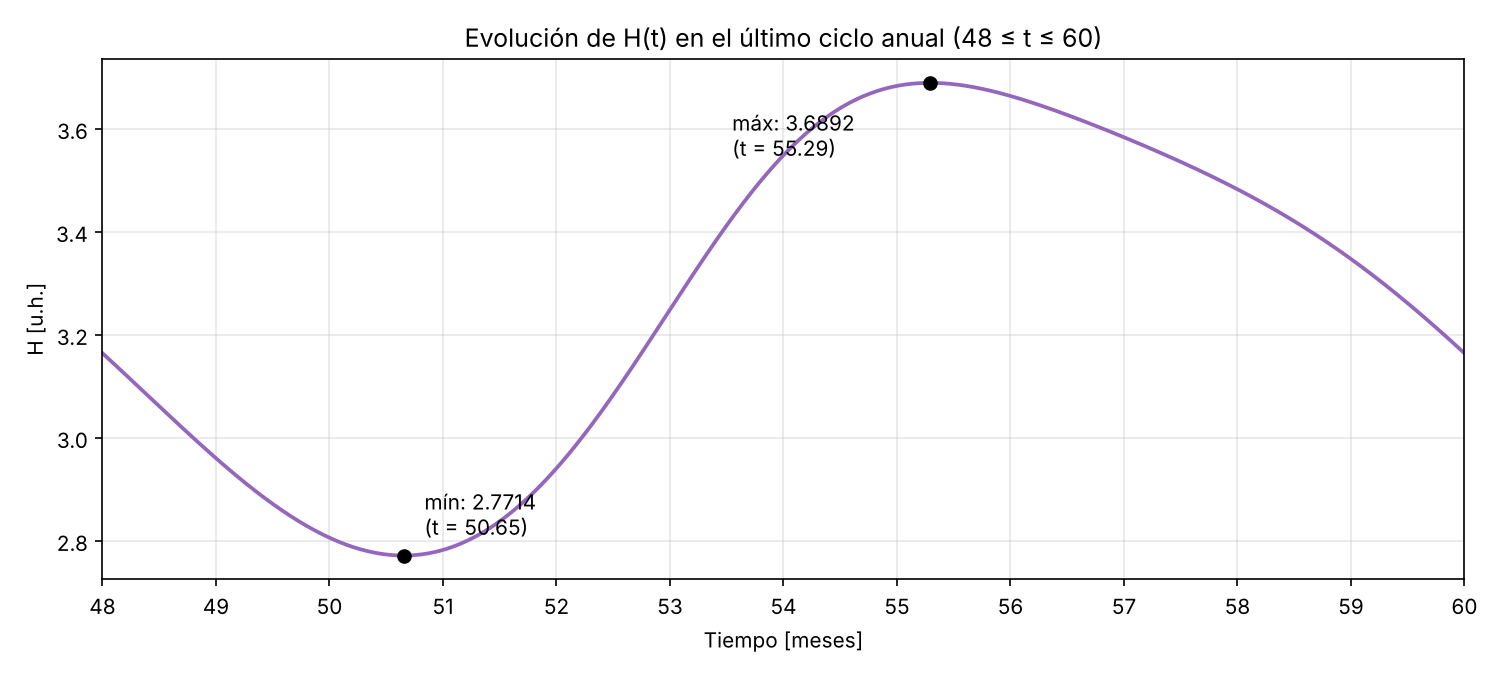
\includegraphics[width=0.75\linewidth]{graficoH.png}
    \caption{Evolución de $H(t)$ para $48 \le t \le 60$ meses.}
    \label{fig:H}
\end{figure}



\begin{figure}[H]
    \centering
    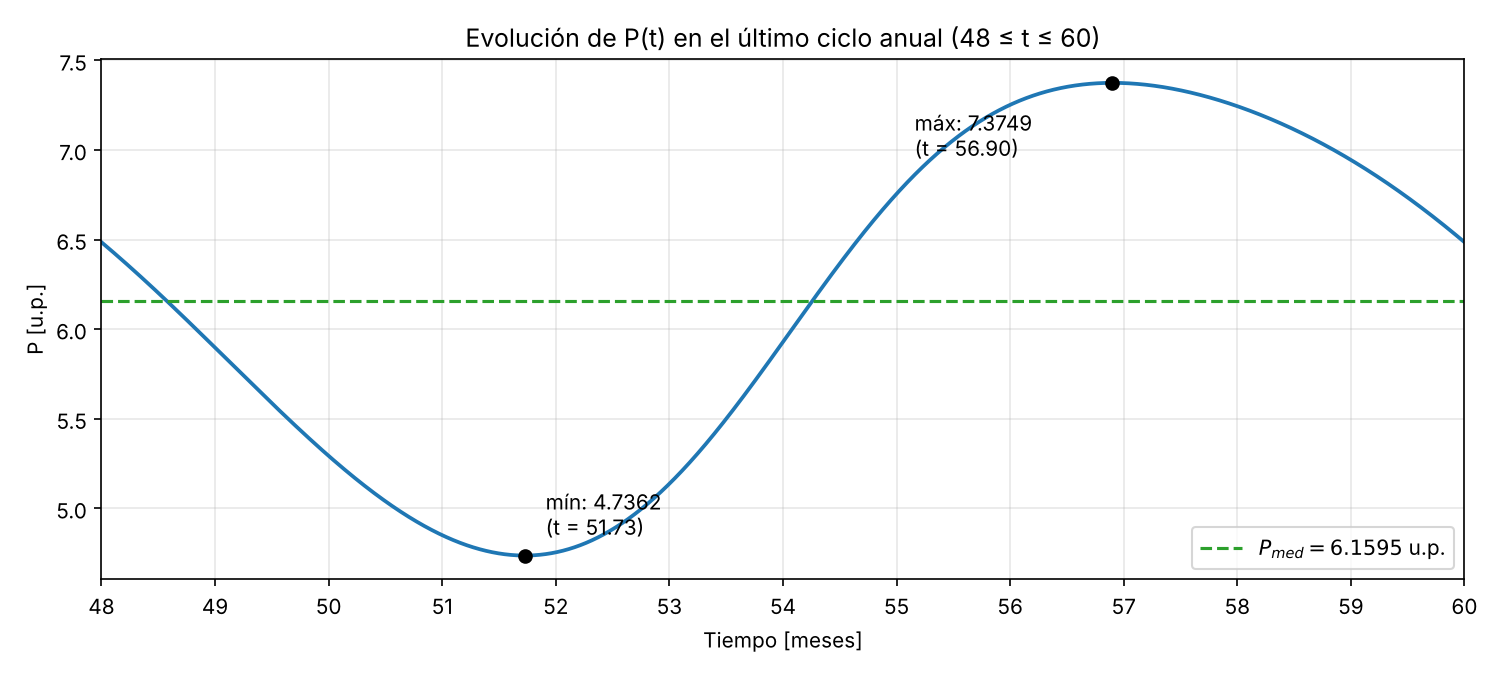
\includegraphics[width=0.75\linewidth]{graficoP.png}
    \caption{Evolución de $P(t)$ para $48 \le t \le 60$ meses.}
    \label{fig:P}
\end{figure}


A partir de la Figura 6, el máximo de la precipitación se alcanza en
$t_{P,\max} = 56.90\ \text{meses}$, con $P_{\max} = 7.3749\ \text{u.p.}$,
$P_{\min} = 4.7362\ \text{u.p.}$ y $P_{\text{med}} = 6.1595\ \text{u.p.}$

Con estos valores, los indicadores resultan:
\begin{itemize}
    \item Severidad estacional: $S_P = \dfrac{7.3749 - 4.7362}{6.1595} = 0.4284$
    \item Desfase temperatura-precipitación: $\Delta t_{TP} = 56.90 - 56.07 = 0.83\ \text{meses}$
\end{itemize}
\subsection{Sensibilidad de los indicadores a los parámetros del modelo}
En esta sección se analizará individualmente la influencia de los parámetros $A$, $\beta$, $\gamma$ y $\sigma$ modificando un parámetro por vez, manteniendo los
restantes en sus valores nominales. Se buscará determinar el comportamiento de los indicadores $SP$ y $\Delta t_{TP}$ calculados sobre el último ciclo anual utilizando los siguientes intervalos:
\begin{center}
\begin{tabular}{ll}
\hline
Parámetro & Intervalo de exploración \\
\hline
$A$ & $0.25$ a $0.60\ \text{mes}^{-1}$ \\
$\beta$ & $0.10$ a $0.30\ \text{u.h.}\,\text{mes}^{-1}\,^\circ\text{C}^{-2}$ \\
$\gamma$ & $0.05$ a $0.20\ \text{mes}^{-1}\,\text{u.p.}^{-1}$ \\
$\sigma$ & $0.40$ a $1.00\ \text{mes}^{-1}$ \\
\hline
\end{tabular}
\end{center}

\subsubsection{Influencia del parámetro $A$}
\begin{figure}[H]
    \centering
    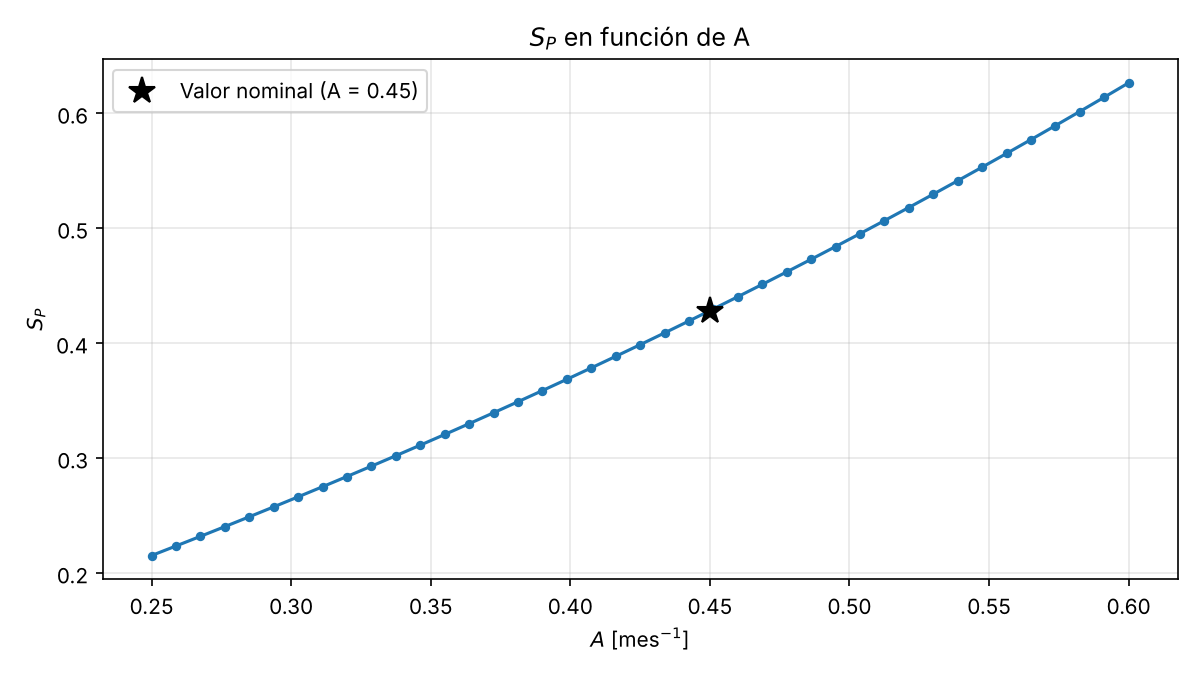
\includegraphics[width=0.75\linewidth]{SP_A.png}
    \caption{ Tendencia de $S_P(A)$}
\end{figure}
\begin{figure}[H]
    \centering
    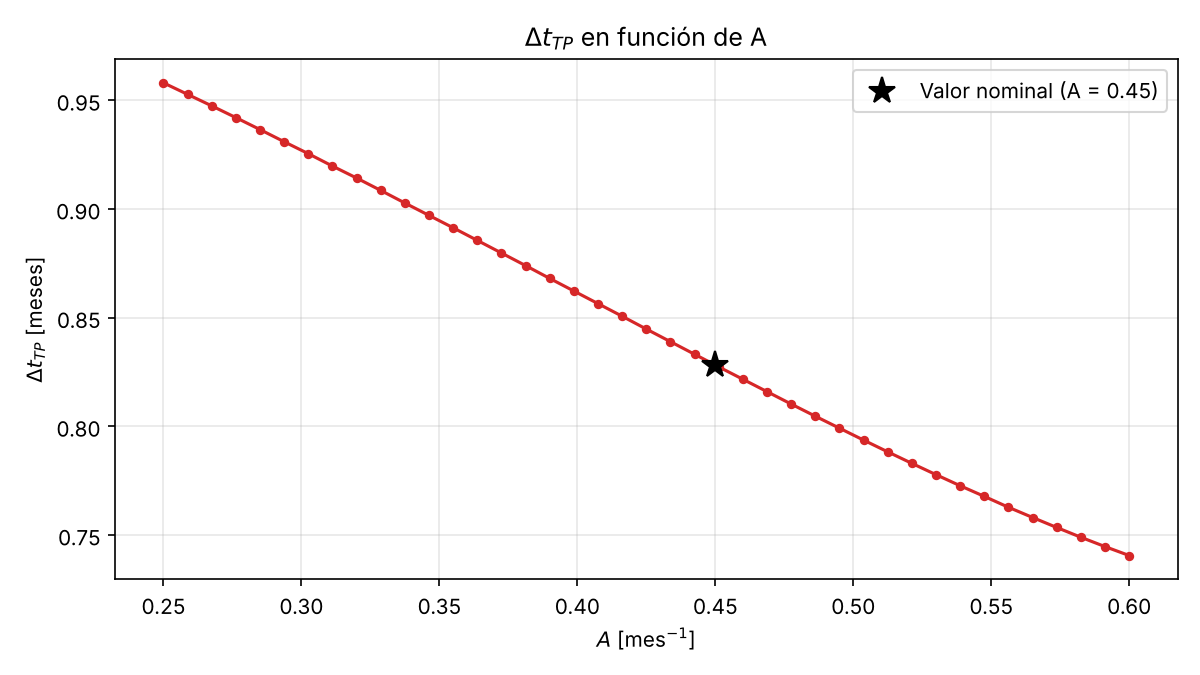
\includegraphics[width=0.75\linewidth]{dtTP_A.png}
    \caption{ Tendencia de $\Delta t_{TP}(A)$}
\end{figure}
Teniendo en cuenta la figura 7, se puede observar que la severidad estacional es creciente en cuanto se incrementa el valor del parámetro A. Por el contrario, la figura 8 muestra que el desfase temperatura-precipitación decrece en cuanto mayor sea A.

Analizando las ecuaciones diferenciales, el parámetro A tiene influencia en la tasa de crecimiento térmico R(t), que está modulada por una excitación estacional de período anual. En esta expresión, A es la amplitud de la modulación estacional y multiplica al término coseno. Como la función coseno varía entre -1 y 1, al incrementar el valor de A aumenta el rango de valores que puede tomar R(t), mientras que el resto de términos y el período de la función coseno no se modifican.

Al haber una mayor amplitud, se intensifica el contraste estacional entre meses de calentamiento y enfriamiento. Esto hace que las precipitaciones también oscilen entre extremos más alejados y explica el crecimiento de su severidad $S_P(A)$.

A su vez, con una A más grande el calentamiento ocurre de forma más intensa y concentrada, y T sube más rápido hasta su pico.
Un cambio de temperatura más fuerte y abrupto lleva a que haya más precipitación. P no tarda tanto en enterarse de que el océano se calentó y su máximo aparece más cerca del de T, explicando el por qué disminuye el indicador $\Delta t_{TP}(A)$.

\subsubsection{Influencia del parámetro $\beta$}
\begin{figure}[H]
    \centering
    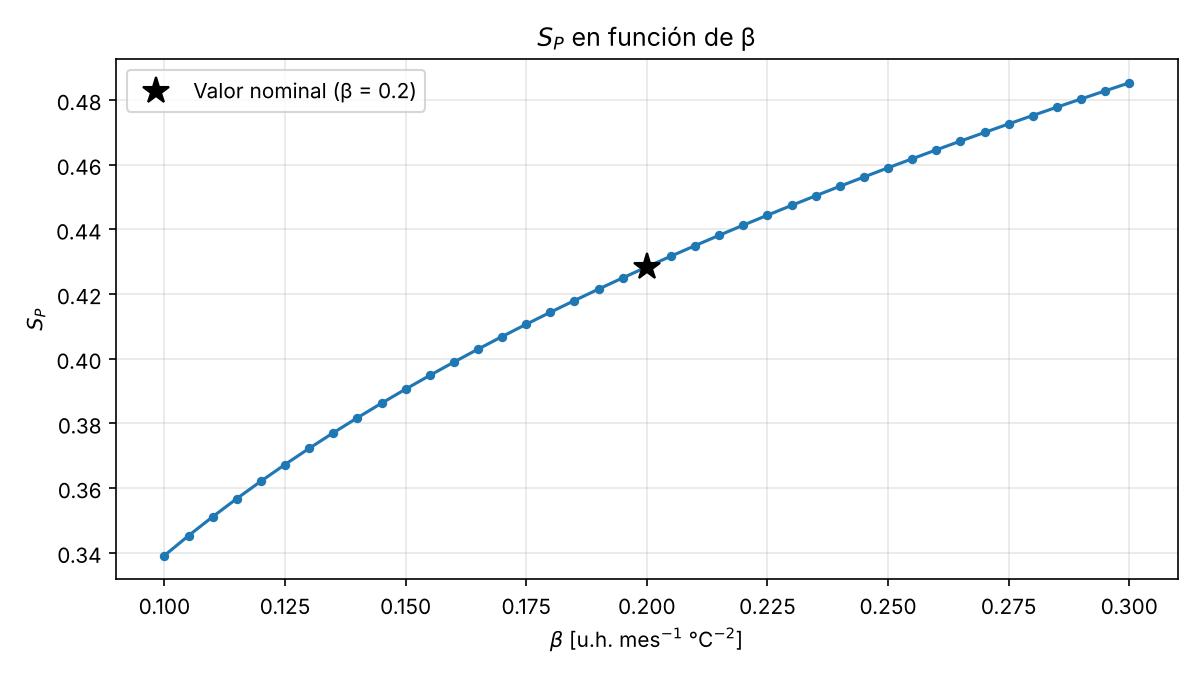
\includegraphics[width=0.75\linewidth]{SP_beta.png}
    \caption{ Tendencia de $S_P(\beta)$}
\end{figure}
\begin{figure}[H]
    \centering
    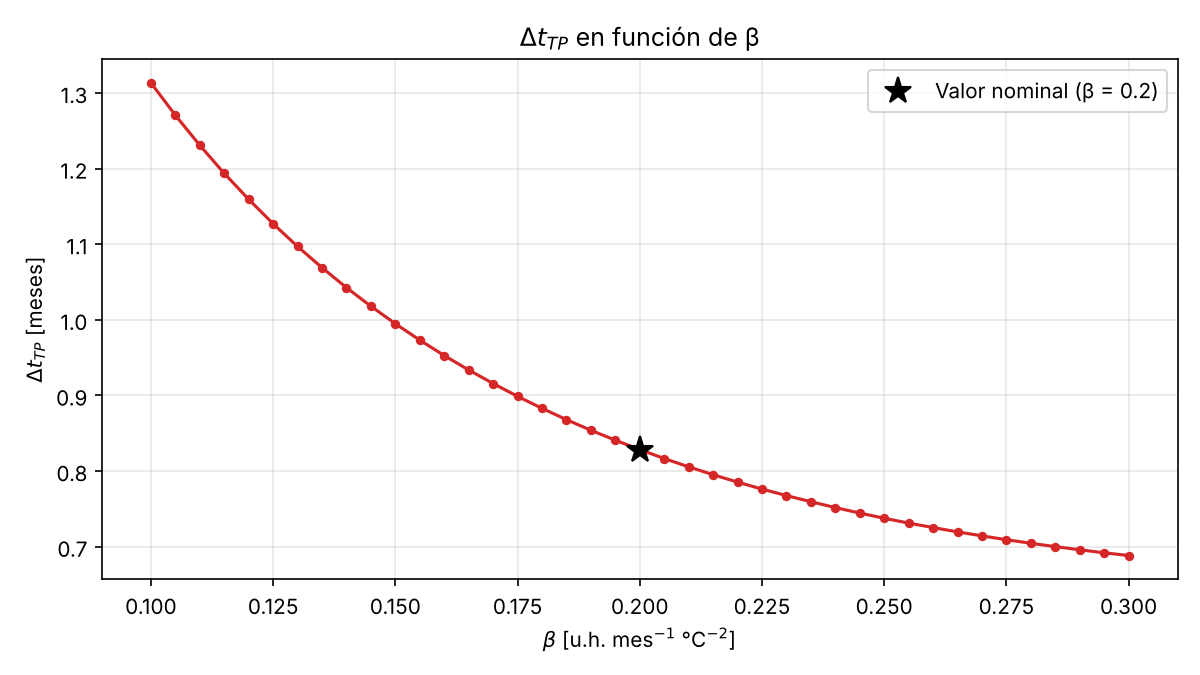
\includegraphics[width=0.75\linewidth]{dtTP_beta.png}
    \caption{ Tendencia de $\Delta t_{TP}(\beta)$}
\end{figure}
A partir de la figura 9, se observa una tendencia creciente para el indicador de severidad cuanto mayor sea el parámetro $\beta$. La figura 10, en cambio, refleja un comportamiento decreciente del desfase temperatura-precipitación.

El parámetro $\beta$ es la eficiencia de evaporación e interviene en la ecuación diferencial que incluye la derivada de la anomalía de humedad en la atmósfera baja $H$. En particular, multiplica el cuadrado de la anomalía de temperatura superficial del mar. Esto da la idea de que al haber una mayor eficiencia de evaporación, aumenta la facilidad con la que se genera humedad a partir de la temperatura superficial del mar. En consecuencia, esto trae más precipitaciones y con ello incrementa su
severidad, como muestra el gráfico del indicador $S_P(\beta)$.

También, al generarse la humedad más rápido, la anomalía P tarda menos en reaccionar al incremento de la temperatura del mar y hace que el desfase entre temperatura-precipitación $\Delta t_{TP}(\beta)$ disminuya.

\subsubsection{Influencia del parámetro $\gamma$}
\begin{figure}[H]
    \centering
    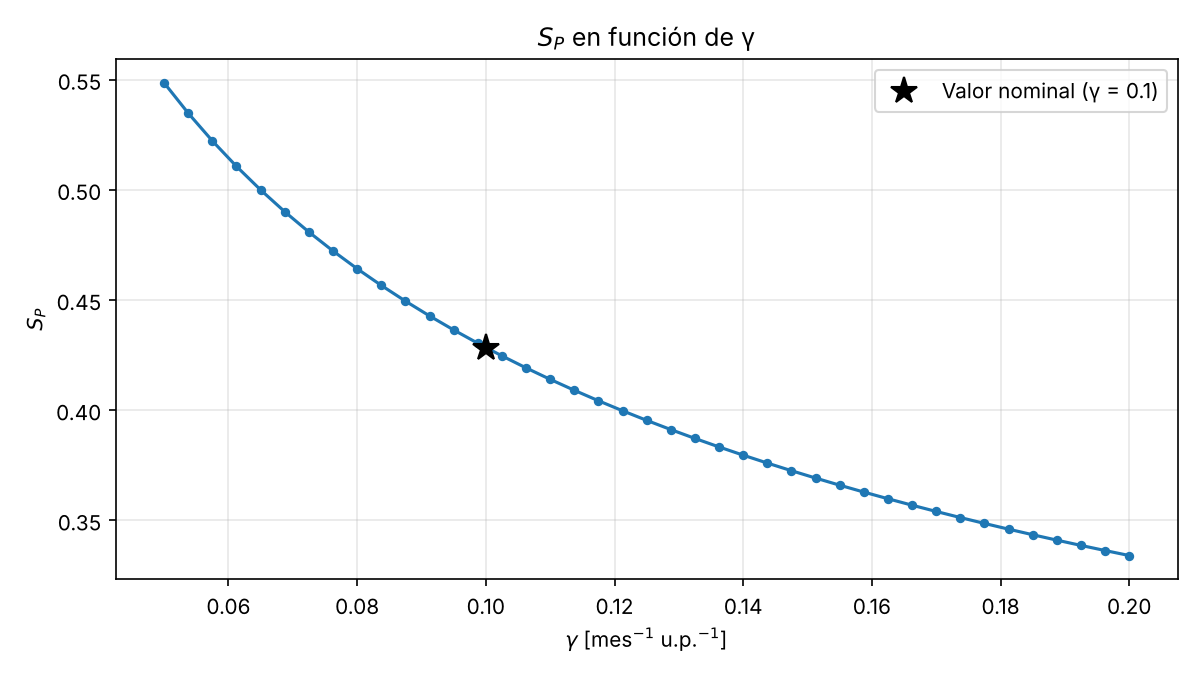
\includegraphics[width=0.75\linewidth]{SP_gamma.png}
    \caption{ Tendencia de $S_P(\gamma)$}
\end{figure}
\begin{figure}[H]
    \centering
    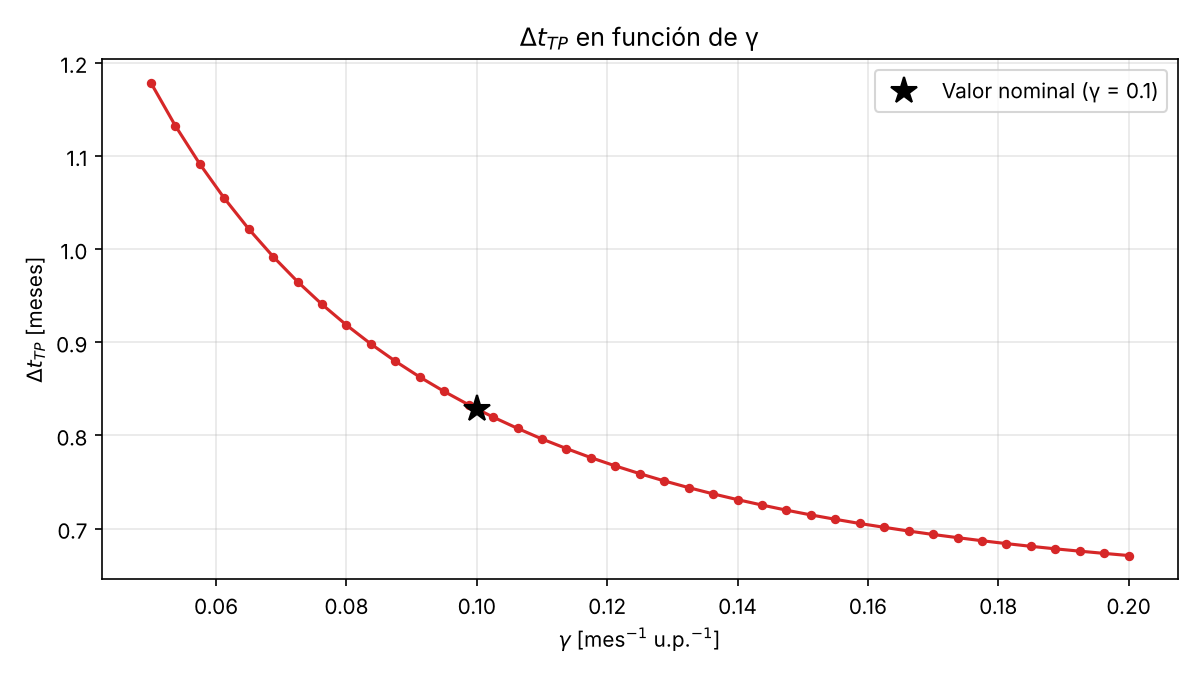
\includegraphics[width=0.75\linewidth]{dtTP_gamma.png}
    \caption{ Tendencia de $\Delta t_{TP}(\gamma)$}
\end{figure}
En ambas figuras 11 y 12 se observa que los indicadores decrecen en cuanto aumenta el valor del parámetro $\gamma$

En cuanto a las ecuaciones diferenciales, $\gamma$ aparece en aquella que incluye la derivada de la anomalía de humedad en la atmósfera baja $H$. En particular, en un término negativo que multiplica dicha anomalía por la variable asociada a las precipitaciones $P$. Este parámetro representa la tasa de consumo de humedad por precipitación, por lo que aumentar su valor significa que cada precipitación consume más humedad. Como el resto de variables del problema no se cambia, el hecho de que la lluvia consuma más humedad hace que quede menos humedad disponible para que pueda llover, por lo que efectivamente las precipitaciones y sus variaciones se reducen, y consigo su severidad $S_P(\gamma)$.

Por otro lado, al consumirse la humedad más rápido, esta alcanza su máximo antes y la precipitación también, por lo que el desfase entre temperatura-precipitaciones baja. Esto confirma la tendencia vista en el gráfico de $\Delta t_{TP}(\gamma)$.

\subsubsection{Influencia del parámetro $\sigma$}
\begin{figure}[H]
    \centering
    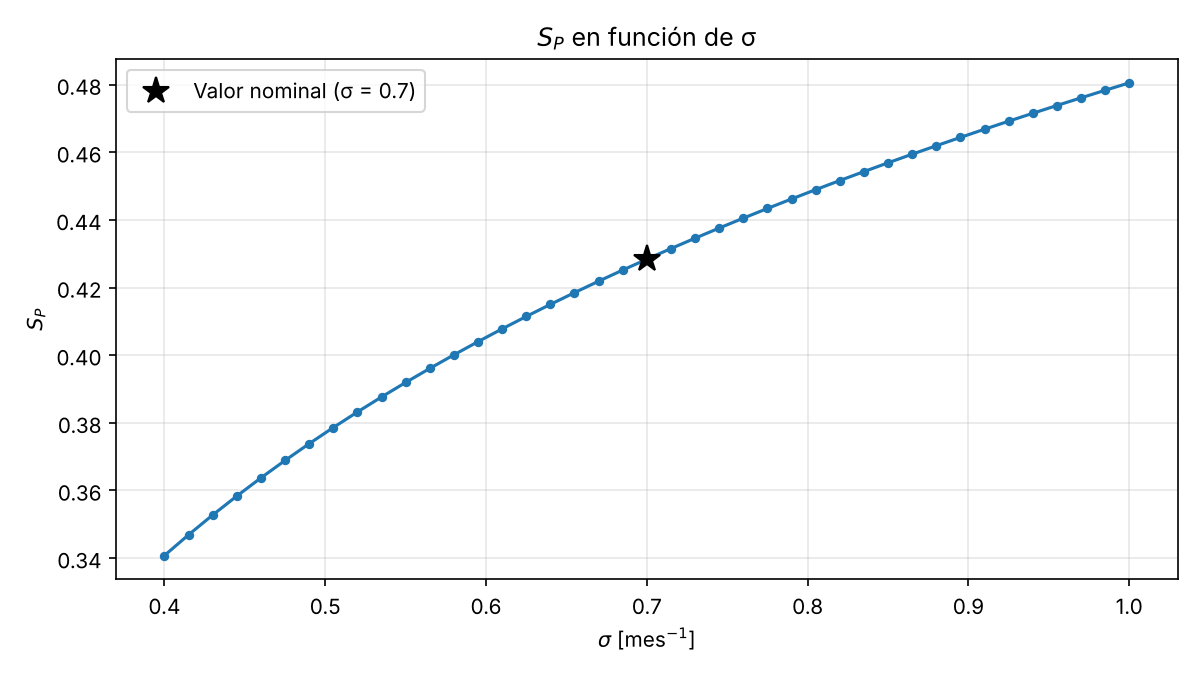
\includegraphics[width=0.75\linewidth]{SP_sigma.png}
    \caption{ Tendencia de $S_P(\sigma)$}
\end{figure}
\begin{figure}[H]
    \centering
    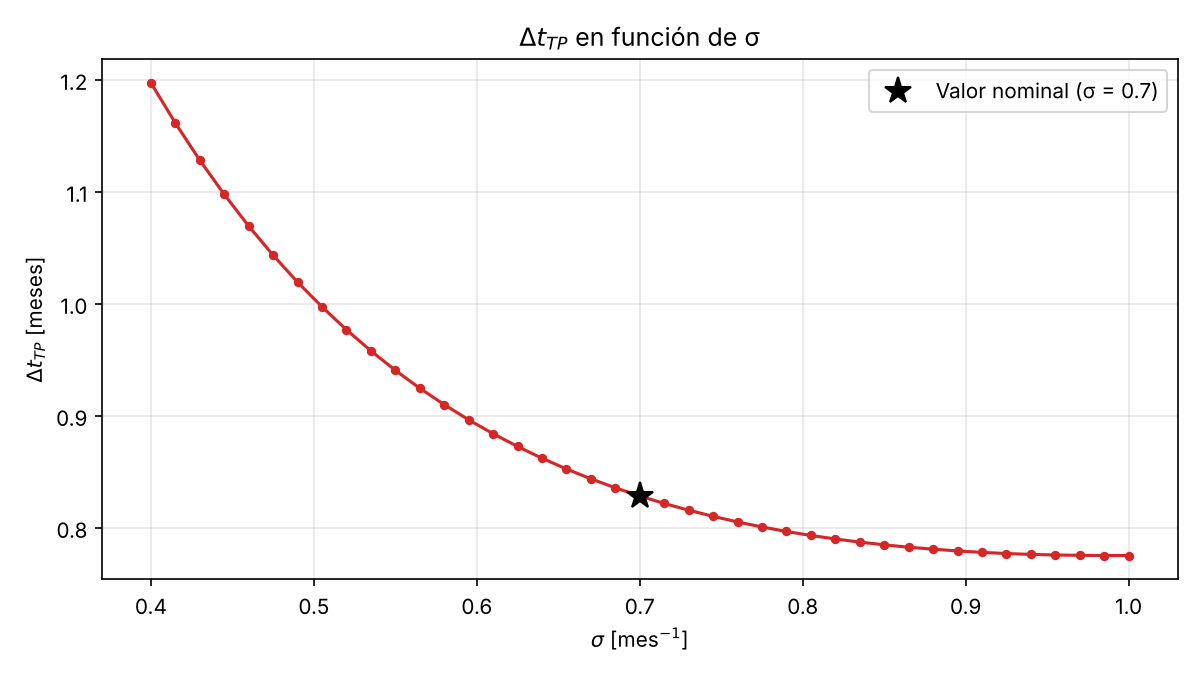
\includegraphics[width=0.75\linewidth]{dtTP_sigma.png}
    \caption{ Tendencia de $\Delta t_{TP}(\sigma)$}
\end{figure}

En la figura 13 se puede observar un comportamiento creciente del indicador $S_P(\sigma)$ cuanto más crece el parámetro, mientras que en la figura 14 la tendencia es la contraria.

El parámetro $\sigma$ representa la tasa de disipación sobre el continente y aparece en la ecuación diferencial que incluye la derivada de la variable asociada a las precipitaciones $P$. En dicha ecuación, aparece multiplicando a esta variable en un término negativo. A priori, se puede decir que un incremento en $\sigma$ significa que las precipitaciones se descargan más rápido a lo largo del continente. Entonces, como las lluvias no se acumulan y desaparecen más rápido, la variable $P$ sigue más de cerca los cambios de la humedad a lo largo del año, por lo que la diferencia entre la temporada de mayores lluvias y la de menos es mayor respecto del promedio, es esperable que su severidad aumente como sugiere el indicador $S_P(\sigma)$.

A su vez, el máximo de la humedad y las precipitaciones se alcanzan ambos con mayor rapidez al haber una mayor zona donde afectan las lluvias. Por lo tanto, tiene sentido que baje el indicador de desfase entre estas dos variables $\Delta t_{TP}(\sigma)$.

\subsection{Maximización de severidad estacional}

\subsection{Comparación de indicadores con parámetros nominales y modificados}